\section{Разработка средства обмена сообщениями}
Чтобы в течение игрового процесса игроки могли взаимодействовать между собой, было
принято решение разработать средство обмена сообщениями (далее <<чат>>). Чат позволяет
игрокам совместно решать поставленные задачи, а также обмениваться опытом за короткий промежуток времени. \par 

Чаты делятся на три типа:
\begin{itemize}
    \item общий - это такой чат, который по умолчанию есть у всех пользователей, из него нельзя выйти, в нем состоят абсолютно все зарегистрированные пользователи, и владельцем этого чата является администратор;
    \item групповой - это такой чат, который состоит из трех и более человек и владельцем которого является либо создатель чата, либо тот человек, которому были выданы соответствующие права;
    \item приватный - это такой чат, который состоит из двух человек.
\end{itemize}

\vspace{1em}

Для разработки чата потребовалось дополнить существующую базу данных, а также продумать процесс 
работы чата и реализовать соответствующие методы. \par 

В процессе проектирования таблиц базы данных была создана схема, изображенная на рисунке \ref{img:bd_schema}

\clearpage

\begin{figure}[h!]
    \centering
    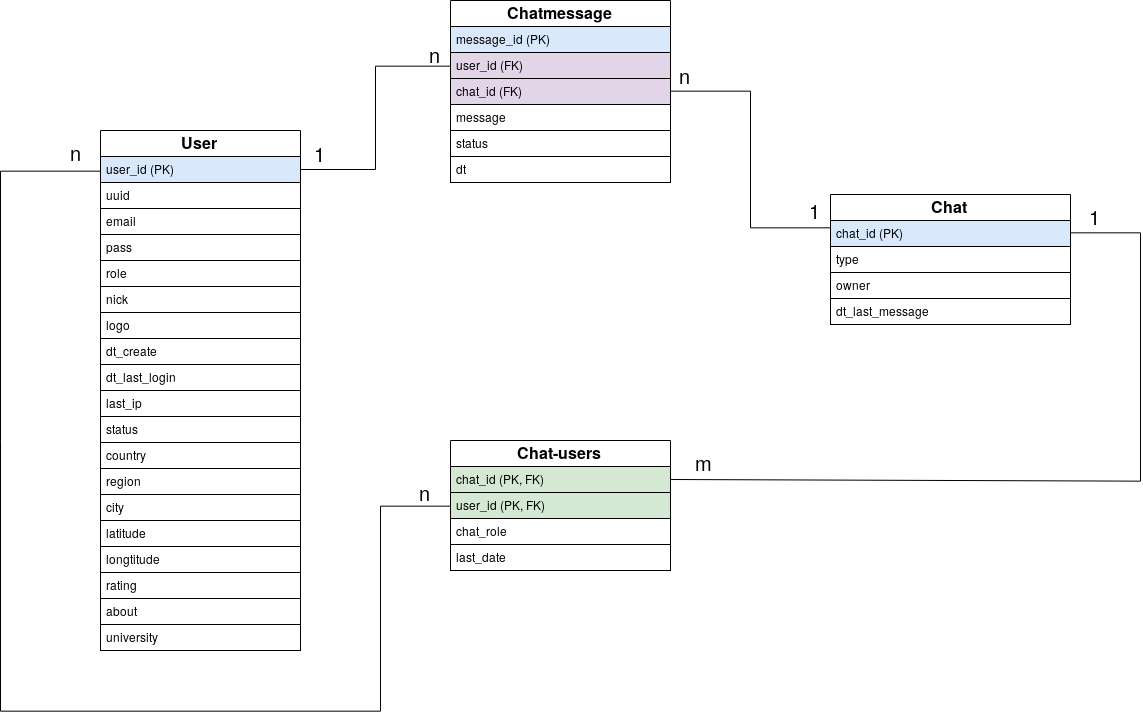
\includegraphics[width=0.9\textwidth]{images/database}
    \caption{Схема базы данных}
    \label{img:bd_schema}
\end{figure}

Далее приведено описание таблиц и их полей. \par 
Таблица <<Chatmessages>> нужна для того, чтобы хранить всю необходимую информацию о сообщениях, и 
имеет следующие поля:
\begin{itemize}
    \item message\_id - хранит идентификатор сообщения;
    \item user\_id - идентификатор пользователя, автор сообщения;
    \item chat\_id - идентификатор чата, в который было отправлено сообщение;
    \item message - текст сообщения;
    \item status - статус сообщение: "прочитано" или "не прочитано";
    \item dt - дата и время отправления сообщения.
\end{itemize}

\vspace{1em}

Таблица <<User>> нужна для того, чтобы хранить информацию о пользователе, и имеет следующие поля:
\begin{itemize}
    \item user\_id - идентификатор пользователя;
    \item uuid - дополнительный строковый идентификатор;
    \item email - почтовый адрес пользователя;
    \item pass - пароль пользователя;
    \item nick - псевдоним, использующийся пользователем в системе;
    \item logo - графическое изображения пользователя;
    \item dt\_create - дата создания пользователя;
    \item dt\_last\_login - время последней активности пользователя;
    \item last\_ip - последний IP-адрес, с которого заходил пользователя;
    \item status - статус пользователя: в сети он или нет;
    \item country - страна проживания пользователя;
    \item region - регион проживания пользователя;
    \item city - город проживания пользователя;
    \item latitude - географическая широта;
    \item longtitute - географическая долгота;
    \item rating - рейтинг пользователя: количество набранных очков.
\end{itemize}

\vspace{1em}

Таблица <<Chat>> нужна для того, чтобы хранить информацию о чате. Имеет следующие поля:

\begin{itemize}
    \item chat\_id - идентификатор чата;
    \item type - тип чата: общий, групповой или приватный;
    \item owner - владелец чата. Изначально им является создатель, но может быть переназначен;
    \item dt\_last\_message - дата последнего отправленного сообщения в чат.
\end{itemize}

\vspace{1em}

Таблица <<Chat-users>> реализует связь <<многие-ко-многим>> между таблицами <<Chat>> и <<User>>. Нужна для того, чтобы
у пользователей была возможность состоять в нескольких чатах, и чтобы каждый чат мог содержать от двух до неопределенного количества
пользователей. Содержит следующие поля:
\begin{itemize}
    \item chat\_id - идентификатор чата;
    \item user\_id - идентификатор пользователя;
    \item chat\_role - роль пользователя в чате.
\end{itemize}

\vspace{1em}

После создания таблиц и их добавления в базу данных был предложен перечень методов для реализации чата, а именно:
\begin{itemize}
    \item создание диалога: иниициализация диалога пользователем в начале общения с другим пользователем или создание группового чата.
    \item отправить сообщения: отправление сообщения в текущий чат;
    \item прочитать сообщение: получение списка всех сообщений в текущем чате, а также меняет их статус с <<не прочитано>> на <<прочитано>>;
    \item показать список диалогов: получение списка всех чатов, в которых состоит пользователь;
    \item редактировать сообщение: исправление текста сообщения, которое уже было отправлено в чат;
    \item удаление сообщения: удаление сообщение из чата, в который оно было отправлено;
    \item ответить на сообщение: выделение сообщения или нескольких сообщений, которые можно переслать с комментарием;
    \item добавить в групповой чат: добавление пользователей в групповой чат администратором;
    \item исключить из группового чата: удаление пользователя из чата администратором чата или же самим пользователем, если он решил покинуть чат;
    \item смена владельца чата: передача прав администрирования чата другому пользователю;
    \item добавить в черный список: добавление в <<черный список>> пользователей, от которых другой пользователь не хочет получать сообщения;
    \item удалить из черного списка: удаление пользователя из черного списка с последующим возвращением прав писать сообщения тому, кто ранее их туда добавил.
\end{itemize}

\vspace{1em}

Для разработки данных методов применялась методология разработки программного обеспечения TDD (Test-Driven Development), которая основывается 
на повторении очень коротких циклов разработки: сначала пишется тест, покрывающий желаемое изменение, затем пишется код, который позволит пройти тест, 
и под конец проводится рефакторинг нового кода к соответствующим стандартам. Данная методология полезна еще и тем, что на данном этапе веб-интерфейс сайта не обладает достаточным функционалом для
тестирования разрабатываемых методов.

Всего было реализовано четыре метода из вышеперечисленных, а именно: отправка, чтение, редактирование и удаление сообщения. По методологии TDD были написаны тесты, а затем сами методы. 

Результат работы представлен на рисунке \ref{img:tests}

\begin{figure}[h!]
    \centering
    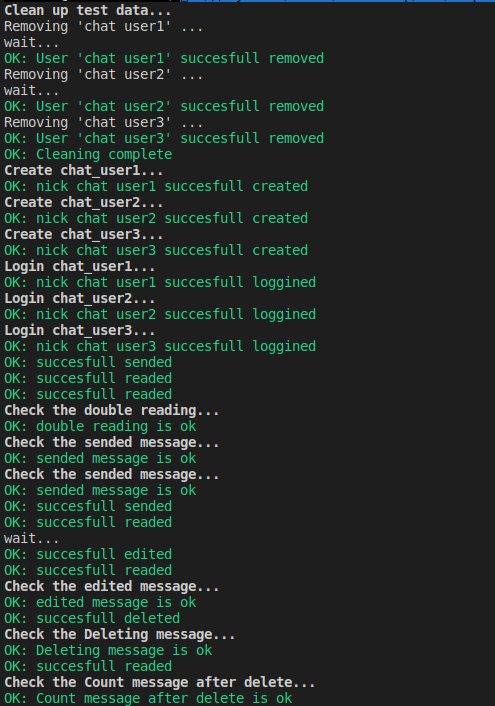
\includegraphics[width=0.7\textwidth]{images/tests}
    \caption{Результат разработки методов для чата по методологии TDD}
    \label{img:tests}
\end{figure}

Эти тесты работают следующим образом: вызывается некоторый метод из API (Application User Interface) с определенными параметрами. Возвращаемое значение метода известно заранее,
поэтому, исходя из этого, можно проводить сравнение полученное значение с ожидаемым. Если они совпадают, тест пройден успешно, если нет, то, соответственно, тест не пройден. 

Рассмотрим один из вызовов тестируемого метода на примере метода chats\_send\_message (отправка сообщения). На рисунке \ref{img:send_msg} реализован тест выходных данных на их соответствие.

\begin{figure}[h!]
    \centering
    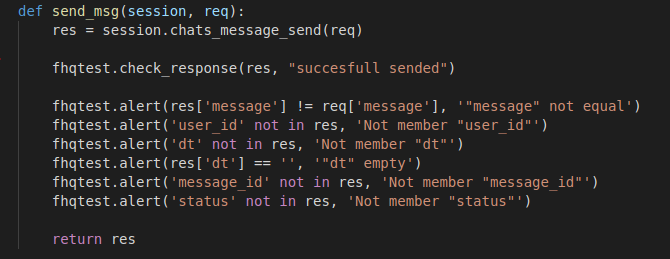
\includegraphics[width=0.9\textwidth]{images/send_msg}
    \caption{Тест выходных параметров}
    \label{img:send_msg}
\end{figure}

Ожидается, что функция chats\_message\_send вернет ответ, который состоит из: отправляемого сообщения, идентификатора пользователя-автора сообщения, времени отправки,
идентификатора сообщения и его статуса. 

Тест взаимосвязанных вызовов представлен на рисунке \ref{img:test_call}.

\begin{figure}[h!]
    \centering
    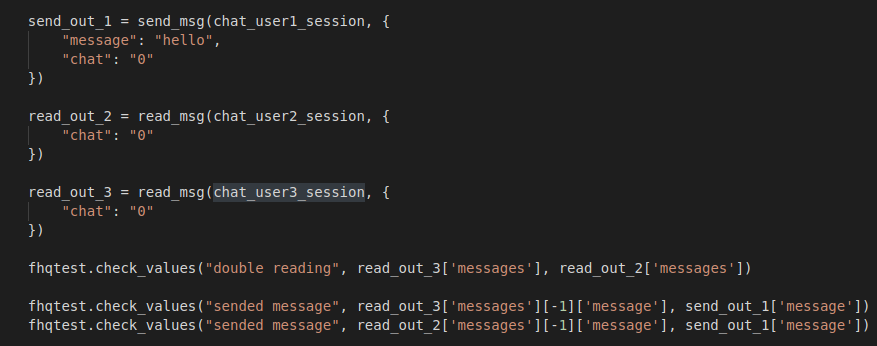
\includegraphics[width=0.9\textwidth]{images/test_call}
    \caption{Тест выходных параметров}
    \label{img:test_call}
\end{figure}

\vspace{15em}

Ожидается, что последнее отправленное сообщение будет тем же самым, что и последнее полученное. 